\documentclass[12pt,a4paper]{report}

% --- Packages ---
\usepackage[utf8]{inputenc}
\usepackage[T1]{fontenc}
\usepackage{geometry}
\geometry{top=1in, bottom=1in, left=1in, right=1in}
\usepackage{graphicx}
\usepackage{xcolor}
\usepackage{hyperref}
\usepackage{titlesec}
\usepackage{tocloft}
\usepackage{fancyhdr}
\usepackage{tabularx}
\usepackage{enumitem}
\usepackage{caption}
\usepackage{float}
\usepackage{tikz}
\usetikzlibrary{shapes,arrows,positioning,trees}
\usepackage{listings}
\usepackage{mdframed}
\usepackage{mathptmx} % Times New Roman equivalent
\usepackage{tcolorbox}
\usepackage{amssymb}
\usepackage{lmodern}
\usepackage{ragged2e}

% --- Questionnaire Custom Commands ---
\newtcolorbox{boxstyle}{
  colback=lightgrey,
  colframe=primary,
  arc=6pt,
  boxrule=0.9pt,
  left=6pt,right=6pt,top=6pt,bottom=6pt
}

\newcommand{\opt}{\(\circ\)}

\newcolumntype{Y}{>{\RaggedRight\arraybackslash}X}
\newcommand{\likertheader}{ & 1 & 2 & 3 & 4 & 5 & 6 & 7 & 8 & 9 & NA \\
\hline}
\newcommand{\likertrow}[1]{#1 & \opt & \opt & \opt & \opt & \opt & \opt & \opt & \opt & \opt &  \\
\hline}

% --- Colors ---
\definecolor{primary}{HTML}{2E5A88}
\definecolor{secondary}{HTML}{4A90E2}
\definecolor{dark}{HTML}{212121}
\definecolor{lightgrey}{HTML}{F5F5F5}

% --- Hyperref Setup ---
\hypersetup{
    colorlinks=true,
    linkcolor=primary,
    filecolor=magenta,      
    urlcolor=secondary,
    pdftitle={PrayasMarked Final Project Report},
}

% --- Custom Header/Footer ---
\pagestyle{fancy}
\fancyhf{}
\fancyhead[L]{\textit{PrayasMarked: NGO Attendance System}}
\fancyhead[R]{\thepage}
\fancyfoot[C]{Department of Computer Engineering}
\renewcommand{\headrulewidth}{0.4pt}
\renewcommand{\footrulewidth}{0.4pt}

% --- Title Page ---
\begin{document}

\begin{titlepage}
    \centering
    \vspace*{0.5cm}
    {\large \textbf{[UNIVERSITY NAME]}} \\
    \vspace{0.2cm}
    {\large \textbf{[COLLEGE NAME]}} \\
    \vspace{1.5cm}
    
    \begin{figure}[h]
        \centering
        \includegraphics[width=4cm]{university_logo.png} % Replace with your uni logo filename
        \caption*{University Logo}
    \end{figure}
    
    \vspace{1cm}
    {\huge \textbf{\textcolor{primary}{PrayasMarked}}} \\
    \vspace{0.5cm}
    {\Large \textbf{NGO Attendance \& Tracking System}} \\
    \vspace{1.5cm}
    
    \begin{mdframed}[backgroundcolor=lightgrey, linecolor=primary, linewidth=1pt]
        \centering
        \vspace{0.3cm}
        \textbf{FINAL PROJECT REPORT} \\
        \text{Submitted for the Course: [Course Name / Code]}
        \vspace{0.3cm}
    \end{mdframed}
    
    \vspace{1.5cm}
    \begin{table}[h]
        \centering
        \begin{tabular}{l l l}
            \textbf{Sr. No.} & \textbf{Team Member Name} & \textbf{Enrollment No.} \\
            \hline
            1 & Jugal Vaghmashi & 21BCE001 \\
            2 & Harshil [Surname] & 21BCE002 \\
            3 & Smit [Surname] & 21BCE003 \\
            4 & Meet [Surname] & 21BCE004 \\
        \end{tabular}
    \end{table}
    
    \vfill
    {\large \textbf{Academic Year: 2025-2026}} \\
    {\large \textbf{Group Number: [XX]}} \\
    
\end{titlepage}

% --- Contents ---
\pagenumbering{roman}
\tableofcontents
\newpage
\listoffigures
\newpage
\listoftables
\newpage

\pagenumbering{arabic}

% --- Chapter 1 ---
\chapter{Introduction}
\section{Motivation}
The inspiration for \textbf{PrayasMarked} originated from observing the operational challenges faced by animal care NGOs and rescue shelters. In many such organizations, tracking the status of rescued animals—from admission (Mark IN) to recovery and eventual release (Mark OUT)—is still handled through fragmented manual records or simple spreadsheets. This lack of a centralized system often leads to:
\begin{itemize}
    \item Difficulty in accessing real-time medical updates for specific animals.
    \item Inefficient coordination between treatment and rehab centers.
    \item Challenges in generating periodic occupancy reports for stakeholders.
\end{itemize}
PrayasMarked aims to bridge this gap by providing a modern, reliable, and user-friendly digital platform tailored for the unique workflows of animal welfare organizations.

\section{Overview of Project}
\textbf{PrayasMarked} is a sophisticated web application designed to handle the end-to-end lifecycle of rescued animals. Built with a focus on Glassmorphism-inspired UI and robust role-based access control, the system allows staff members to log admissions, update medical records, and manage transfers between different care stages seamlessly. Key features include a dynamic species engine, automated treatment queues, and a comprehensive admin dashboard for high-level monitoring.

\section{Market Survey}
During the planning phase, we analyzed several existing solutions for shelter management. The following table summarizes our findings:
\begin{table}[H]
    \centering
    \caption{Market Survey Comparison}
    \begin{tabularx}{\textwidth}{|l|X|l|}
        \hline
        \textbf{System Name} & \textbf{Pros} & \textbf{Cons} \\
        \hline
        ShelterBuddy & Enterprise features, wide adoption. & Steep learning curve, expensive. \\
        RescueGroups.org & Free tools, API support. & Dated interface, complex setup. \\
        \textbf{PrayasMarked} & \textbf{Mobile-first, modern UI, specific to NGO workflows.} & \textbf{Newer platform, limited integrations.} \\
        \hline
    \end{tabularx}
\end{table}

% --- Chapter 2 ---
\chapter{Details of Tools}
\section{Brief Description of Facilities Available}
Our project utilizes a modern full-stack architecture to ensure scalability and a premium user experience.
\begin{itemize}
    \item \textbf{Frontend:} Vanilla JavaScript, CSS3, and HTML5. We opted for a custom Single Page Application (SPA) architecture to maintain full control over the Glassmorphism aesthetic and animations.
    \item \textbf{Backend:} Node.js with Express. A RESTful API manages authentication and data processing.
    \item \textbf{Database:} MongoDB (Mongoose) provides a flexible schema for varying animal medical records.
\end{itemize}

\section{Comparison with Other Tools}
\begin{table}[H]
    \centering
    \caption{Tool Comparison Table}
    \begin{tabularx}{\textwidth}{|l|X|l|}
        \hline
        \textbf{Feature} & \textbf{PrayasMarked (JS/Node)} & \textbf{Alternatives (React/Firebase)} \\
        \hline
        Learning Curve & Low - Uses standard web technologies. & Moderate - Requires learning hooks/JSX. \\
        Bundle Size & Extremely lightweight. & Larger dependencies. \\
        Real-time Data & Socket.io implementation. & Firebase Firestore (Built-in). \\
        Customization & High control over every DOM element. & Component-driven constraints. \\
        \hline
    \end{tabularx}
\end{table}

% --- Chapter 3 ---
\chapter{Project Planning and Preparation}
\section{Paper-Pen Designs}
The initial architectural design of \textbf{PrayasMarked} began with low-fidelity wireframes sketched on paper. These blueprints focused on two core areas: the "Admission Admission Form" and the "Admin Intelligence Dashboard." The primary design goal was to minimize the number of clicks required for staff working in stressful, on-field environments.

\begin{figure}[H]
    \centering
    \includegraphics[width=0.45\textwidth]{paper_design_1.jpg}
    \includegraphics[width=0.45\textwidth]{paper_design_2.jpg}
    \caption{Manual sketches of the Admission workflow and Dashboard layout}
    \label{fig:paper_designs}
\end{figure}

The sketches emphasized a "Mobile-First" approach, ensuring that critical data like Job IDs and Treatment Status were prominently displayed even on small screens.

\section{Persona Development}
\begin{itemize}[label=--]
    \item \textbf{Persona 1: Volunteer Staff (Rahul)}
    \begin{itemize}
        \item Age: 22
        \item Role: Rescuer / Caretaker
        \item Goal: Quick entry of new rescues and updating medical status.
    \end{itemize}
    \item \textbf{Persona 2: Admin / Manager (Dr. Sharma)}
    \begin{itemize}
        \item Age: 45
        \item Role: Shelter Head
        \item Goal: Monitoring total occupancy and exporting reports for audit.
    \end{itemize}
\end{itemize}

\section{Scenario Description}
"A rescue call arrives at 2 AM. Rahul brings in a puppy with a leg injury. He opens PrayasMarked on his phone, enters the breed details using the smart species engine, marks the treatment status as 'Emergency', and saves. Dr. Sharma sees this update on her dashboard immediately and coordinates the senior vet."

\section{Use Case Description}
\begin{figure}[H]
    \centering
    \begin{mdframed}[linecolor=primary]
        \textbf{Use Case: Record New Admission} \\
        \textbf{Actor:} Staff Member \\
        \textbf{Pre-condition:} Staff is logged in. \\
        \textbf{Main Flow:} 1. Navigate to Admission. 2. Select Species. 3. Enter Medical Remarks. 4. Submit. \\
        \textbf{Post-condition:} Animal record is added to DB and dashboard counter increments.
    \end{mdframed}
\end{figure}

% --- Chapter 4 ---
\chapter{Project Features}
\section{Integrated Features Comparison}
All features developed by the team have been integrated into a cohesive platform:
\begin{description}
    \item[Auth Engine:] JWT-based secure login and Role Based Access Control (RBAC).
    \item[Admission Control:] Handled via a dynamic form with nested subspecies selection.
    \item[Tracking Module:] Capability to move animals between treatment and rehabilitation centers.
    \item[Analytics Suite:] Real-time counters and progress bars for occupancy tracking.
\end{description}

\section{Design Review Link}
The complete design and source repository can be accessed for review here: \\
\vspace{0.2cm}
\textbf{Github Repository:} \href{https://github.com/jugal-ahir/PrayasMarked}{https://github.com/jugal-ahir/PrayasMarked}

\section{Screen Connectivity and Linking}
The application screens are linked through a unified navigation drawer. Figure \ref{fig:screens} illustrates how different modules communicate:
\begin{itemize}
    \item \textbf{Login $\rightarrow$ Dashboard:} Main entry point upon authentication.
    \item \textbf{Dashboard $\rightarrow$ Admissions:} Direct shortcut for entering new animal data.
    \item \textbf{Dashboard $\rightarrow$ Analytics:} Detailed view of occupancy trends.
    \item \textbf{In-App Navigation:} Side-drawer allows switching between "Treatment Center" and "Rehab Center" sections.
\end{itemize}

\section{Hierarchical Task Analysis (HTA)}
Below is the HTA for the core task of "Managing Animal Admission \& Care Progression":

\begin{figure}[H]
\centering
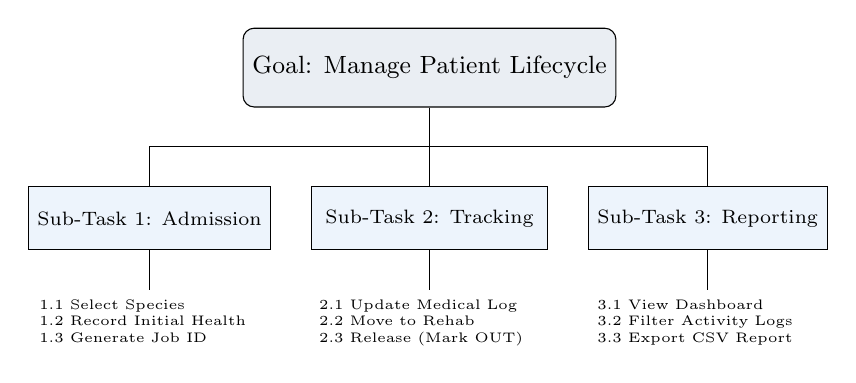
\begin{tikzpicture}[
  node distance=1cm and 0.5cm,
  box/.style={draw, rectangle, rounded corners, fill=primary!10, text centered, minimum width=3.5cm, minimum height=1cm, font=\small},
  subbox/.style={draw, rectangle, fill=secondary!10, text centered, minimum width=3cm, minimum height=0.8cm, font=\scriptsize},
  line/.style={draw, -latex'}
]

% Goal
\node[box] (goal) {Goal: Manage Patient Lifecycle};

% Level 1
\node[subbox, below=1cm of goal] (st2) {Sub-Task 2: Tracking};
\node[subbox, left=of st2] (st1) {Sub-Task 1: Admission};
\node[subbox, right=of st2] (st3) {Sub-Task 3: Reporting};

% Level 2
\node[font=\tiny, below=0.5cm of st1, text width=2.8cm, align=left] (st11) {1.1 Select Species\\1.2 Record Initial Health\\1.3 Generate Job ID};
\node[font=\tiny, below=0.5cm of st2, text width=2.8cm, align=left] (st21) {2.1 Update Medical Log\\2.2 Move to Rehab\\2.3 Release (Mark OUT)};
\node[font=\tiny, below=0.5cm of st3, text width=2.8cm, align=left] (st31) {3.1 View Dashboard\\3.2 Filter Activity Logs\\3.3 Export CSV Report};

% Connectors
\draw (goal.south) -- ++(0,-0.5) -| (st1.north);
\draw (goal.south) -- ++(0,-0.5) -| (st2.north);
\draw (goal.south) -- ++(0,-0.5) -| (st3.north);

\draw (st1.south) -- (st11.north);
\draw (st2.south) -- (st21.north);
\draw (st3.south) -- (st31.north);

\end{tikzpicture}
\caption{Hierarchical Task Analysis for PrayasMarked}
\end{figure}

% --- Chapter 5 ---
\chapter{Difficulties Encountered and Resolved}
\section{Description of Debugging and Resolution}
\begin{enumerate}
    \item \textbf{Jugal Vaghmashi (Auth Persistence):} Maintaining secure session persistence in a pure Vanilla JS frontend without page reloads was complex. \textit{Resolution:} Implemented HttpOnly cookies combined with a central state manager to synchronize UI components across the app.
    \item \textbf{Harshil (Cross-Browser Blur):} Achieving a consistent Glassmorphism blur effect across mobile browsers. \textit{Resolution:} Integrated specific vendor-prefixed CSS backdrop-filters and provided semi-transparent fallbacks for older devices.
    \item \textbf{Smit (Aggregation Performance):} Calculating real-time occupancy across multiple species efficiently. \textit{Resolution:} Developed optimized MongoDB aggregation pipelines using \$facet to fetch multiple counters in a single database call.
    \item \textbf{Meet (Responsive Data Tables):} Handling long activity logs on mobile screens. \textit{Resolution:} Implemented a "Mobile-First" toggle that switches from table view to a card-based layout for smaller viewports.
\end{enumerate}

% --- Chapter 6 ---
\chapter{Real Life Implementation Perspectives}
\section{Problems and Proposed Solutions}
\begin{itemize}
    \item \textbf{Problem: Spotty Internet Connectivity.} Volunteers often work in areas with poor network coverage. \\
    \textit{Solution:} We propose implementing Progressive Web App (PWA) features that allow offline data entry, which syncs to the server once a connection is re-established.
    \item \textbf{Problem: Hardware Limitations.} NGOs often rely on donated or older hardware. \\
    \textit{Solution:} The light-weight nature of Vanilla JS ensures that the app remains performant even on low-RAM devices.
\end{itemize}

\section{Security and Privacy Issues}
The system stores sensitive volunteer emails and animal locations. Key security layers include:
\begin{itemize}
    \item \textbf{JWT Signature:} Ensures that API requests cannot be forged.
    \item \textbf{RBAC:} Standard volunteers cannot modify historical logs, preserving the integrity of records.
    \item \textbf{Environment Security:} API keys and database strings are never hardcoded and are managed via secure environment variables.
\end{itemize}

\section{Rules and Regulation Requirements}
Compliance with local NGO registration laws requires detailed audit trails for animal movement. PrayasMarked provides a comprehensive, unalterable "Activity Log" that satisfies most governmental documentation requirements for rescue missions.

% --- Chapter 7 ---
\chapter{References}
\begin{itemize}
    \item [1] MDN Web Docs: CSS Backdrop-filter Documentation. \href{https://developer.mozilla.org}{developer.mozilla.org}
    \item [2] Mongoose Documentation: Aggregation Framework and Pipelines. \href{https://mongoosejs.com}{mongoosejs.com}
    \item [3] JWT.io: Understanding JSON Web Tokens.
    \item [4] Nielsen Norman Group: Heuristic Evaluation for Modern Interfaces.
\end{itemize}

% --- Chapter 8 ---
\chapter{Project Video and Deliverables}
The complete project demonstration video, including feature explanations and team voiceovers, is hosted on the cloud for accessibility: \\
\vspace{0.5cm}
\textbf{Google Drive Share Link:} \href{https://drive.google.com/drive/folders/your-video-link-here}{https://drive.google.com/drive/folders/your-link} \\
\vspace{0.2cm}
\textbf{GitHub Source Link:} \href{https://github.com/jugal-ahir/PrayasMarked}{https://github.com/jugal-ahir/PrayasMarked} \\
\textit{Video Duration: 6 Minutes | Format: 1080p MP4}

\newpage
\appendix
\chapter{Questionnaire for Survey}

\begin{center}
{\LARGE \textbf{PrayasMarked User Experience Survey}}\\
{\small \textit{Project Lead: Jugal Vaghmashi}}
\end{center}

\vspace{0.4cm}

% PART 1
\section*{Part 1: Usage Context}
\begin{boxstyle}
\textbf{1.1 Your Role:} \opt Admin \quad \opt Volunteer \quad \opt Vet/Medical Staff

\textbf{1.2 Usage Frequency:}
\begin{itemize}[label=\opt,noitemsep]
\item Daily
\item Few times a week
\item Occasionally
\end{itemize}

\textbf{1.3 Primary Use Case:}
\begin{itemize}[label=\opt,noitemsep]
\item Animal Admission (Mark IN)
\item Medical Tracking
\item Rehabilitation Tracking
\item Release (Mark OUT)
\item Dashboard/Reports
\end{itemize}

\textbf{1.4 Preferred Device:} \opt Mobile \quad \opt Tablet \quad \opt Desktop
\end{boxstyle}

% PART 2
\section*{Part 2: Core Features Evaluation}
\begin{boxstyle}
\begin{tabularx}{\textwidth}{|Y|*{10}{c|}}
\hline
\likertheader
\likertrow{Adding new animal records (Mark IN) is intuitive}
\likertrow{Updating animal health status is efficient}
\likertrow{Species/Sub-species selection is comprehensive}
\likertrow{The system handles rapid data entry well}
\likertrow{Reviewing historical activity logs is straightforward}
\end{tabularx}
\end{boxstyle}

% PART 3
\section*{Part 3: Interface \& Navigation}
\begin{boxstyle}
\begin{tabularx}{\textwidth}{|Y|*{10}{c|}}
\hline
\likertheader
\likertrow{The Glassmorphism UI is visually clean}
\likertrow{Forms are logically structured for on-field use}
\likertrow{Navigation between Dashboard and Centers is smooth}
\likertrow{The Side Navigation Drawer is easy to access}
\likertrow{Toast notifications provide clear action feedback}
\end{tabularx}
\end{boxstyle}

% PART 4
\section*{Part 4: Domain Understanding}
\begin{boxstyle}
\begin{tabularx}{\textwidth}{|Y|*{10}{c|}}
\hline
\likertheader
\likertrow{Terms like Mark IN/OUT are clear for NGO workflow}
\likertrow{Treatment vs Rehab stages match real-world process}
\likertrow{Medical remarks are displayed clearly across the logs}
\likertrow{Real-time counters help in shelter capacity planning}
\likertrow{The system labels (Species, Remarks etc) are relevant}
\end{tabularx}
\end{boxstyle}

% PART 5
\section*{Part 5: Reliability \& Security}
\begin{boxstyle}
\begin{tabularx}{\textwidth}{|Y|*{10}{c|}}
\hline
\likertheader
\likertrow{System gives clear validation/error messages}
\likertrow{Data entry feels secure and tamper-proof}
\likertrow{The application performs consistently without lag}
\likertrow{Login/Logout processes are secure and fast}
\likertrow{You trust the system for long-term digital records}
\end{tabularx}
\end{boxstyle}

% PART 6
\section*{Part 6: Learning \& Efficiency}
\begin{boxstyle}
\begin{tabularx}{\textwidth}{|Y|*{10}{c|}}
\hline
\likertheader
\likertrow{The system is easy to learn for new volunteers}
\likertrow{Tasks can be completed faster than paper methods}
\likertrow{Minimal technical training is required to start}
\likertrow{CSV export saves significant reporting time}
\likertrow{Overall system improves NGO operational efficiency}
\end{tabularx}
\end{boxstyle}

\vspace{0.4cm}
\noindent\textbf{Suggestions / Additional Comments:}\\[0.2cm]
\rule{\textwidth}{0.4pt}

\end{document}
